%           %experimenting with svn-multi

\svnkwsave{$RepoFile: siminos/froehlich/slice.tex $}
\svnidlong {$HeadURL$}
{$LastChangedDate$}
{$LastChangedRevision$} {$LastChangedBy$}
\svnid{$Id$}


\section{\Reducedsp}
\label{sect:reducedStateSp}

\begin{bartlett}
I made a wrong mistake.
\bauthor{Yogi Berra}
\end{bartlett}

\noindent
Now that we know what a symmetry of a dynamical system is, how
(or why) can it actually be used?

Suppose you are observing turbulence in a pipe flow, or your
defibrillator has a mesh of sensors measuring electrical currents that
cross your heart. Here you see a pattern, and there you see a pattern
that seems much like the first one. How ``much like the first one?'' Or
you have a precomputed pattern, and are sifting through the turbulent
data set for something like it. Think of the first pattern (represented
by a point {\slicep} in the \statesp) as a
`template'\rf{rowley_reconstruction_2000,rowley_reduction_2003} or a
`reference state' and use the symmetries of the flow to slide and rotate
the `template' until it overlays the second pattern, \ie, act with elements of
the symmetry group \Group\ on the template \statesp\ point ${\slicep} \to
{\LieEl}{\slicep}$ until the distance between the two patterns, measured
in a bilinear norm of \refsect{def:innerProduct},
    \PC{recheck, is the unitary case different,
	(one does need $2 \Re \,\braket{\sspRed}{\slicep}$).
	If so, restrict consideration to subgroups of \SOn{n}.}
\bea
|\ssp - {\LieEl}{\slicep}|^2
    &=& |\sspRed - \slicep|^2
		\,=\,
   \braket{\sspRed - \slicep}{\sspRed - \slicep}
%\\ |\ssp|^2 - 2\,\Re\braket{\sspRed}{\slicep} +|\slicep|^2
\,,
    \label{minDistance}
\eea
is minimized. Here $\sspRed$ is the point on the group orbit
of $\ssp$,
\beq
\ssp=\LieEl \sspRed
\,,
\ee{sspOrbit}
closest to the template. Rather than blindly sliding one pattern over the
other, we determine the group rotation `angles' $\gSpace =
(\gSpace_1,\gSpace_2,\cdots\gSpace_N)$ by solving the extremum condition
	\PC{to select minima, need 2nd partials}
\bea
0 &=&
\frac{\partial ~~}{\partial \gSpace_a} |\ssp - \LieEl\slicep|^2
	\continue
  &=& \braket{\sspRed - \slicep}{\sliceTan{a}}
    \,,\qquad
	  \sliceTan{a} = \Lg_a \slicep
\,,
\label{PCsectQ}
\eea
where $\ssp \in \pS$ is a point in the full \statesp, and  the group
elements \refeq{FiniteRot} of Lie group $\Group$ are represented  by
$\LieEl=\exp(\gSpace \cdot \Lg)$.
By the antihermiticity of $\Lg$, \refeq{antiHerm},  we have
$\braket{\slicep}{\sliceTan{a}}=0$, and the transformation parameters
$\gSpace$ for which the state $\ssp$ is closest to the template
$\slicep$ are given by $N$ conditions
\beq
\braket{\sspRed}{\sliceTan{a}} =0
    \,\qquad
\sspRed = \LieEl(\gSpace) \ssp
\,.
\ee{PCsectQ0}

A given compact group orbit intersects a slice at least twice, and
possibly many times, so we need a prescription for how to
pick a unique \reducedsp\ point as the representative of the entire group
orbit.

The extremal distance condition \refeq{PCsectQ1} is a condition that
closest point $\sspRed$ in the group orbit of $\ssp$ lies in a
$(d\!-\!N)$-dimensional hyperplane normal to the group action tangent
space $\sliceTan{}$ at template point $\slicep$. If the two patterns are
close, their group orbits will be nearly parallel, and for a smooth flow
this tangent plane will be transverse to all group orbits of $\ssp$ in a
neighborhood of \slicep.

However, we will be bolder, and show next that for a generic
template $\slicep$ (\ie, any $\slicep$ whose group orbit is $N$-dimensional),
the slice hyperplane cuts across {\em all} group orbits in \pS.

For this \slice\ to be operationally useful, we first must show that a
\slice\ \refeq{PCsectQ1} cuts the group orbit of every point in the full
\statesp.


If $\ssp$ is the invariant subspace \refeq{def:centralizer}, its group
orbit is itself and the distance $|\sspRed - \slicep|$ is fixed.

As a generic group orbit is a curved $N$-dimensional manifold embedded in
the \statesp, several values of $\gSpace$ might be local extrema of the
distance function \refeq{minDistance}; we only care about those that are
local {\em minima}, for which all the eigenvalues of tensor
\refeq{PCinflPoint} are positive. The physically most interesting one is
presumably the closest one, the absolute minimum of \refeq{minDistance}.
It does not matter whether the group is compact, for example $\On{n}$, or
noncompact, for example the Euclidean group that underlies the generation
of spiral patterns\rf{Barkley94}; in either case any group orbit has
one or several locally closest passages to the template state.
    \PC{recycle this:
Here we describe symmetry reduction by the
{\em {\mslices}} of
Cartan\rf{CartanMF,FelsOlver98,FelsOlver99,OlverInv}.
    }

For
example, group orbits of \SOn{2}\ are topologically circles, and their
projections have maxima, minima and inflection points as extrema.
In order to ensure that we are looking at local minima, we will have to
check the local curvature, \ie, the eigenvalues and eigenvectors of the
symmetric matrix $[N\!\times\!N]$ matrix of second derivatives
of distance,
\beq
\frac{\partial^2}
     {\partial \gSpace_a \partial \gSpace_b}
        |\sspRed - \slicep|^2
    =
%  - \braket{\Lg_a e^{\gSpace \cdot \Lg} \ssp}{\sliceTan{b}}=
  - \braket{\groupTan_a(\sspRed)}{\sliceTan{b}}=
  \braket{\sspRed}{\dual{\Lg}{}_a {\Lg}{}_b\slicep}
\ee{PCinflPoint}


The distance surface $|\sspRed - \slicep|$ can have inflection points,
    \PC{Are we only interested in Laplace-Beltrami operator on the
    group manifold
    \\
    \(
    \frac{\partial^2 ~~}{\partial \gSpace^2} |\sspRed - \slicep|^2 =
    - \braket{\groupTan(\sspRed)}{\sliceTan{}} =
    \braket{\sspRed}{\dual{\Lg} \cdot {\Lg}\,\slicep}
    \)
    }
What role do they play? They are non-generic, but if we consider distance
to local minima at successive instants of a trajectory, coalescence of
nearby minima, maxima pairs cannot be avoided. At the instant of
coalescence the denominator in \refeq{SF:sliceEas} goes through a simple
pole, and the integrated trajectory within slice might jump.



                                                    \exerbox{exer:PCsectionCLe}
                                                    \exerbox{exer:SO2rotAngle}



The basic idea behind symmetry reduction is to define an equivalence
relation on the \statesp\ where two points are equivalent if they are in
the same group orbit of the symmetry group. With any trajectory in the
full \statesp\, $\ssp(\tau)$, we can associate with it a new `\reducedsp'
trajectory, $\bar{\sspRed}(\tau)$, which is the equivalence class of the
full trajectory at any time (\ie\ $\ssp(\tau) \in \bar{\sspRed}(\tau)$
for each $\tau$). Knowing only the \reducedsp\ trajectory, it is not
possible to reconstruct the full space trajectory; additional information
is needed to determine which point of the group orbit is in the original
trajectory.

If a unique representative from an equivalence class is chosen, then
every point in the equivalence class is expressible as a group element
acting on this point. If a unique representative, denoted $\sspRed$, is
chosen from each equivalence class, then to recover the full space
trajectory all that is needed is $\LieEl(\tau)$, the group element needed
to rotate the representative $\sspRed(\tau)$ of the equivalence class to
$\ssp(\tau)$ (\ie\ $\ssp(\tau)=\LieEl(\tau) \sspRed(\tau)$).



                                                \exerbox{exer:SO2cSect}
                                                \exerbox{exer:mslicesInv}


\example{\CLe\ rotation angle.}{\label{exam:CLErotAngle}
To show how the rotation into the \slice\ is computed, consider first the \cLe. There is only one infinitesimal generator for the \SOn{2} symmetry group, so the \reducedsp\ trajectory is given by $\sspRed=\LieEl(\gSpace) \ssp$ where $\gSpace$ is such that $\braket{\sspRed}{\sliceTan{}}=0$. Substituting the \SOn{2}\ Lie algebra generator \refeq{CLfLieGen} and  a finite angle \SOn{2} rotation \refeq{CLfRots} acting on a 5-dim\-ens\-ion\-al space \refeq{eq:CLeR} into the slice condition \refeq{PCsectQ1} yields the explicit formula for $\gSpace$:
\beq
    \braket{\ssp}{\sliceTan{}}\cos\gSpace+\braket{\groupTan_{}(\ssp)}{\sliceTan{}} \sin\gSpace=0
\ee{SL:CLEsliceRot}
\[
     \tan\gSpace= - \frac{\braket{\ssp}{\sliceTan{}}}
                      {\braket{\groupTan_{}(\ssp)}{\sliceTan{}}}
\]
\[
    (x_1 x_2'-x_2 x_1'+y_1 y_2' -y_2 y_1')\cos\gSpace
    + (x_1 x'_1+x_2 x'_2+y_1 y'_1+y_2 y'_2)\sin\gSpace
=0
\,.
\]
%    \PC{Stefan, I think you have to explain that, just as in the
%    case of Poincar\'e sections, one keeps track of only oriented
%    crossings, \ie, a circle has only on section in a \slice,
%    not two. That should give you a precise $\pi$ rotation rule
%    for singularity crossing.}
Note that if \gSpace\ is a solution, so is $\gSpace+\pi$. If either of the inner products in \refeq{SL:CLEsliceRot} is nonzero then there are exactly two $\gSpace$.
This formula is particularly simple, as in this example the group
acts only through $m=0$ and $m=1$ representations; in general
the `phases' $\gSpace_a$ have to be computed numerically.

    }%end \example{\CLe\ rotation angle

\SFIG{CLEreduced}
{}{
A typical $\{y_1,y_2,z\}$ plot of the reduced \cLf\ strange attractor
with initial point
$(x_1, x_2, y_1, y_2, z) = (1, 2, 3, 1, 2)$ in the slice normal to $\sliceTan{}=(1,0,0,0,0)$. Contrast this plot with \reffig{fig:CLEx2y1z},
and note the apparent discontinuities in the reduced flow.
    }{fig:CLErx2y1z}


	\ifarticle
	\else

%     \Private{
%\noindent{\bf Predrag -
%July 19, Aug 12 2009; Sep 19 2010}
%    }


%%%%%%%%%%%%%%%%%%%%%%%%%%%%%%%%%%%%%%%%%%%%%%%%%%
% computed by PCunrot.nb
\SFIG{ProblemsPill} %PCunrot}
{}{
{\Mslices}, finite time steps version: a
trajectory started on the \slice, with $\ssp_1^{(0)}
=0$, evolves for a finite time to a \statesp\ point with a
non-zero $\hat{\ssp}_1^{(1)}$. The {\em entire} \statesp\ is then
rotated (the `frame is moved') so that the equivalent point
on the circle lies on the \slice, $\ssp_1^{(1)} =0$.
Thus after every finite time step followed by a rotation the
trajectory returns to the 4$\dmn$ $\ssp_1 =0$
\reducedsp.
}
{fig:PCunrot}
%%%%%%%%%%%%%%%%%%%%%%%%%%%%%%%%%%%%%%%%%%%%%%%%%%

\refFig{fig:PCunrot} illustrates the {\mslices},
finite time version.
    \PC{Draw your own \refFig{fig:PCunrot}
        - need to draw a longer segment of the initial trajectory,
        to make it clearer that the whole segment is rotated.
       }

%
%%%%%%%%%%%%%%%%%%%%%%%%%%%%%%%%%%%%%%%%%%%%%%%%%
\exercise{\SOn{2}  rotation angle:}{\label{exer:SO2rotAngle}
Continue the discussion of \refexam{exam:SO2irrepst} and write down the formula for $\gSpace$ for a Fourier expansion of a periodic function. Show that now the \slice\ condition is a polynomial in $\cos\gSpace$, $\sin\gSpace$, and that, depending on the magnitudes of the Fourier series terms, the group orbit may traverse a slice arbitrarily many times.
    \PC{is it still true that the rotation is by $\pi$?}
    } %end \SOn{2}  rotation angle.

\exercise{Determination of group invariants by the {\mslices}:
    }{ \label{exer:mslicesInv}
Show that the $d-N$ \reducedsp\ coordinates determined by the {\mslices} are independent group invariants, and that the {\mslices} allows the determination of (in general non-polynomial) invariants of the group action by a simple  algorithm that works well in high-dimensional \statesp s.
    }

\solution{exer:mslicesInv}
{Determination of group invariants by the {\mslices}:}{
(To be written by Stefan: read and understand relevant parts of Fels and
Olver\rf{FelsOlver98,FelsOlver99,OlverInv}, Siminos\rf{SiminosThesis})
    }

	\fi%end article switch



\subsection{Dynamics in the slice}
\label{sect:MovFrameODE}

Now that we have shown these slices can be used for the entire {\statesp}, our next objective is to investigate
what the equations of motion look like for the \reducedsp\ trajectories.

The \reducedsp\ trajectory is given by $\ssp(\tau)=\LieEl(\tau) \sspRed(\tau)$. Differentiating both sides with respect to time and setting $\velRed=\frac{d \, \sspRed}{d \, \tau}$ we find that,
\[
\vel(\ssp)=\dot{\LieEl} \, \sspRed+\LieEl \, \velRed(\sspRed) \]
\[
\vel(\LieEl \, \sspRed)=\dot{\LieEl} \, \sspRed+\LieEl \, \velRed(\sspRed) \]
\[
\vel=\velRed + \LieEl^{-1} \, \dot{\LieEl} \, \sspRed
\,.
\]
The product of the inverse of the Lie group element and its time derivative give the group tangent at the point:
$\LieEl^{-1}\dot{\LieEl}=e^{-\gSpace \cdot \Lg} \,
\frac{d ~~}{d \, \tau} e^{\gSpace \cdot \Lg}=\dot{\gSpace}\cdot \Lg$, leaving us with the equation for the velocity of the reduced flow in the slice:
\beq
\velRed(\sspRed)=\vel(\sspRed)-\dot{\gSpace}(\sspRed)\cdot \groupTan(\sspRed).
\ee{eq:redVel}

Equation \refeq{eq:redVel} tells us that the velocity in the slice is the difference between the velocity in the full space and the portion in the direction of the group tangent, or, conversely, the velocity in the full space is the sum of the velocity in the slice and the velocity normal to it, along the group tangent. The component of the velocity in the direction of the group orbit is removed to leave only that part which is in the slice.

This equation is true for any factorization $\ssp(\tau)=\LieEl(\tau) \sspRed(\tau)$, and provides no information on how to calculate $\gSpace$, which depends on the choice of the slice.
Let $\sliceTan{a}$ be the group tangents \refdef{def:slice} at the slice fixing point. When we add on the restrictions of our linear slices \refdef{def:slice}, we find that $\gSpace$ must satisfy the system of equations:
\beq
\braket{\velRed(\sspRed)}{\sliceTan{a}}
=\braket{\vel(\sspRed)}{\sliceTan{a}}
 -\braket{\dot{\gSpace}\cdot \groupTan(\sspRed)}{\sliceTan{a}}=0
\label{eq:slicecondition}
\eeq
for each group tangent $\sliceTan{a}$ at the slice fixing point. $\SOn{2}$ has a single group tangent resulting in the explicit system of equations:
\bea
\dot{\gSpace}(\sspRed) &=& \frac{\braket{\vel(\sspRed)}{\sliceTan{}}}
               {\braket{\groupTan(\sspRed)}{\sliceTan{}}}
\continue
\velRed(\sspRed) &=& \vel(\sspRed)
   -\dot{\gSpace}(\sspRed) \cdot \groupTan(\sspRed).
\label{eq:so2reduced}
\eea


    \ifarticle
    \else


 %                                                   \exerbox{exer:CLEsmall-x1x2}
 %                                                   \exerbox{exer:csectionCLeODE}
 %                                                   \exerbox{exer:csectionPhase}
    \PC{still have to derive the general case: ``
Let $\sliceTan{}$ be a vector normal to the plane of the slice. Then the dynamics within the slice are given by
\bea
\dot{\gSpace_a}(\sspRed) &=& \frac{\braket{\vel(\sspRed)}{\sliceTan{a}}}
               {\braket{\groupTan(\sspRed)}{\sliceTan{}}}
\continue
\velRed(\sspRed) &=& \vel(\sspRed)
   -\dot{\gSpace}(\sspRed) \cdot \groupTan(\sspRed)
\label{SF:sliceEas}
\eea
where $\velRed(\sspRed)$ is the velocity in the slice.
    ''}


%%%%%%%%%%%%%%%%%%%%%%%%%%%%%%%%%%%%%%%%%%%%%%%%%%
 File: infMF.xfig
\SFIG{ProblemsPill} %infMF}
{}{
Method of moving frames, infinitesimal formulation.
}
{fig:infMF}
%%%%%%%%%%%%%%%%%%%%%%%%%%%%%%%%%%%%%%%%%%%%%%%%%%

    \PC{Draw your own \reffig{fig:infMF}.
        }
                                                        \exerbox{exer:csectionReduced}
    \PC{
A more elegant derivation is given in
\refrefs{rowley_reconstruction_2000,rowley_reduction_2003}.
    }


%
%%%%%%%%%%%%%%%%%%%%%%%%%%%%%%%%%%%%%%%%%%%%%%%%%%%%%%%%%%%%%%%%%%
% CLEpcSect.png computed by  CLEfinal.nb (repo: vaggelis)
% CLEpcSect2.png computed by CLEfinal.nb (repo: vaggelis)
\begin{figure}[ht]
\begin{center}
(a) % 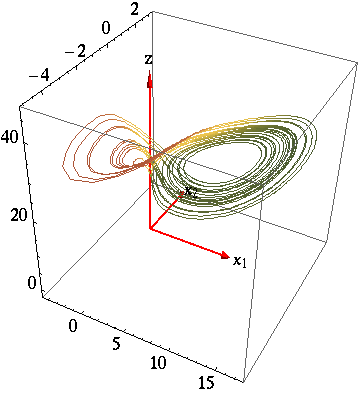
\includegraphics[width=0.40\textwidth]{CLEpcSect}
(b) %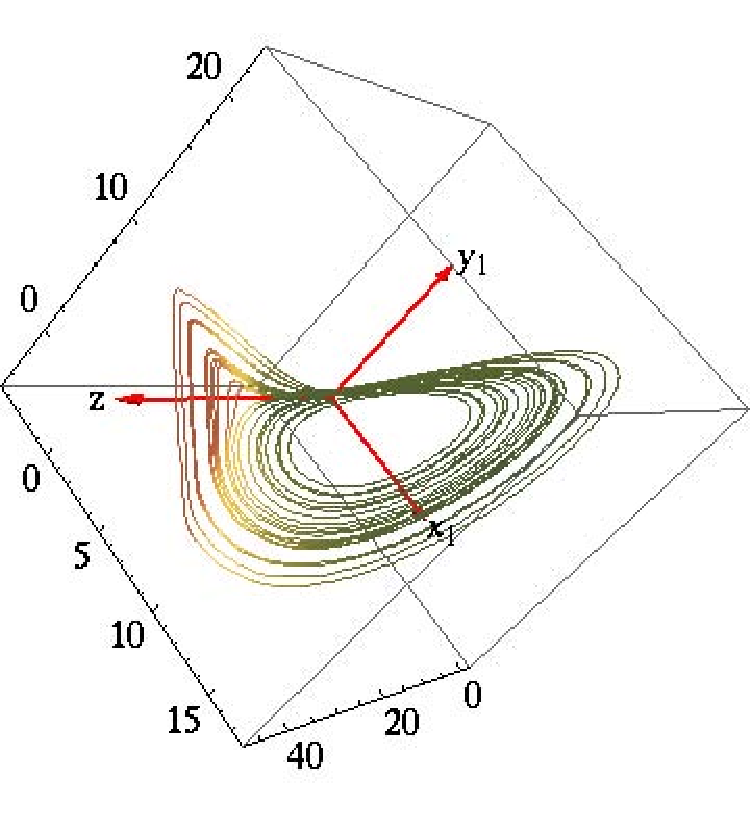
\includegraphics[width=0.43\textwidth]{CLEpcSect2}
\end{center}
\caption{
Method of moving frames, \slice\ fixed by a point on an
\reqv\ group orbit, $\sspRed = \ssp_{\REQB{}1}$. The strange
attractor of \reffig{fig:CLEx1x2z} in the \reducedsp\
of \refeq{EqMotionMovFramePC}:
(a) $\{x_1,x_2,z\}$ projection,
(b) $\{x_1,y_1,z\}$ projection.
Color-coding indicates $(\hat{\ssp} \cdot \hat{\sspRed})_4$
where $\hat{.}$ stands for unit vector, with green indicating values
of the inner product close to $1$ and brown indicating values
close to $0$.
    }
\label{fig:CLEpcSect}
\end{figure}
%%%%%%%%%%%%%%%%%%%%%%%%%%%%%%%%%%%%%%%%%%%%%%%%%%%%%%%%%%%%%%%%
%
A long time trajectory of \refeq{EqMotionMovFramePC} with
$x^*$ on the \reqv\ \REQB{1} group orbit is shown in
\reffig{fig:CLEpcSect}.
                                                        \exerbox{exer:PCsectionCLe}
    \PC{draw your own \reffig{fig:CLEpcSect}:\\
        * Mark $\ssp_{\REQB{}1}$ \\
        * Draw stable eigenvector of $\ssp_{\REQB{}1}$\\
        * State value of $\ssp_{\REQB{}1}$ somewhere
        }


%%%%%%%%%%%%%%%%%%%%%%%%%%%%%%%%%%%%%%%%%%%%%%%%%%
% computed by PCunrot.nb
\SFIG{ProblemsPill} %PCunrot1}
{}{
Method of moving frames, continuous time version, for the
$\slicep=(0,1,0,0)$,
$x_1=0,\;x_2>0$, \slice. The strange attractor of
\reffig{fig:CLEx1x2z} in the \reducedsp,
$\{x_2,y_2,z\}$ projection exhibits a discontinuity at
$x_2=0$.
}
{fig:PCunrot1}
%%%%%%%%%%%%%%%%%%%%%%%%%%%%%%%%%%%%%%%%%%%%%%%%%%

The method encounters singularities in
subsets of \statesp\rf{SiminosThesis}.
                                                    \exerbox{exer:csectionCLe}
A typical trajectory is shown in \reffig{fig:PCunrot1}.

    \fi %end of article switch
	
	
\section{\Slice\ singularities}
\label{sect:sliceSing}

Looking back at equation \refeq{eq:so2reduced}, we see that the \mslices\ potentially introduces singularities to the flow. When the group tangent of a point is in the slice, $\braket{\groupTan(\sspRed)}{\sliceTan{}}$ is zero. Hence  $\dot{\gSpace}(\tau)$ is not defined and as a consequence neither is the velocity in the slice. These singularities do not exist in the full space and are entirely artifacts of the \mslices.

	\ifarticle
	\else
	\PC{text to be eliminated}
In \refsect{sect:reducedStateSp} we noted that the distance surface
\refeq{PCinflPoint} can have inflection points.
What role do they play? They are non-generic, but
if we consider projections of a successive instants of a trajectory
$f(\gSpace)=\braket{e^{\gSpace(t) \cdot \Lg} \ssp(t)}{\slicep}$, coalescence of
nearby minima, maxima pairs cannot be avoided. At the instant of coalescence
the denominator in \refeq{SF:sliceEas} goes through a simple pole,
and the integrated trajectory within slice jumps. Our next task is
to compute the size of the jump.
    \PC{`` from the principal value of the integrated velocity field on a trajectory through this singularity.'' Stefan, take it from here.}
    \PC{could it be that inflections are generic only for \SOn{2},
        but of higher codimension and thus not encountered
        by 1$d$ time trajectory for higher-dimensional Lie groups?}


%If $\ssp(\tau)$ is a trajectory in full {\statesp}, then the
 %\reducedsp\ flow $\sspRed(\tau)$ goes through a singularity when
 %$\braket{\groupTan_{}(\sspRed^*)}{\sliceTan{}}=0$
%at time $\tau=0$, $\sspRed^* = \sspRed(0)$.
%The angle $\gSpace^*$ for rotating a point into the slice must satisfy
 %   \PC{Isn't some of this already worked out in \refexam{exam:CLErotAngle}?
  %      You should refer to already derived results, rather than repeating
   %     the same text}
%\bea
%0             &=&
%\braket{\ssp}{\sliceTan{}}\cos(\gSpace^*) +
%\braket{\groupTan_{}(\ssp)}{\sliceTan{}}\sin(\gSpace^*)
%    \continue
%\tan(\gSpace^*) &=&
%-{\braket{\ssp}{\sliceTan{}}}/{\braket{\groupTan_{}(\ssp)}{\sliceTan{}}}
% \,.
%\label{SF:SO2angleRot}
% \refeq{SF:SO2angleRot}
%\eea
%This equation has two solutions
%$\{\sspRed^*=\LieEl(\gSpace^*)\ssp, \LieEl(\gSpace^*+\pi)\ssp\}$
%unless both $\braket{\sspRed^*}{\sliceTan{}}$
%and $\braket{\groupTan_{}(\sspRed^*)}{\sliceTan{}}$ are zero,
%in which case any angle works (this is exactly the situation
%the trajectory is in when it passes through a singularity
%$\ssp^*$).

%Consider $\gSpace(\tau)$ approaching the singularity value
%$\gSpace^*$ as $\tau \rightarrow 0$.
%The trajectory is smooth, so it can be approximated by the linear
%term in the Taylor expansion,
%$
%\ssp(\tau)=\sspRed^*+\vel^*\tau+O(\tau^2)
%\,,\qquad
%\vel^* = \vel(\sspRed^*)
%    \,.
%$
%    \PC{Stefan had ``
%$\ssp(\tau)=\ssp(0)+\vel(0)\tau+\Mvar(\period{})\frac{\tau^2}{2}$ where $\Mvar$ is the stability matrix and $\period{}$ is between $0$ and $\tau$.
%    '' This looks wrong to me. In any case, the order ${\tau^2}{2}$ term is
%    not used.
% -\frac{\braket{\ssp(0)+\vel(0)\tau
% +\Mvar(\period{})\frac{\tau^2}{2}}{\sliceTan{a}}}{
% \braket{\Lg(\ssp(0)+\vel(0)\tau+\Mvar(\period{})\frac{\tau^2}{2})}{\sliceTan{}}}
%    }
%Hence as $\tau \rightarrow 0$,
%\bea
%\tan(\gSpace)
% = -\frac{\braket{\ssp}{\sliceTan{}}}{\braket{\groupTan_{}(\ssp)}{\sliceTan{}}}
%&\rightarrow&
%-\frac{\braket{\sspRed^*+\vel^*\tau}{\sliceTan{}}}
%{\braket{\Lg(\sspRed^*+\vel^*\tau)}{\sliceTan{}}}
%    \continue
%\tan(\gSpace^*) &=&
%     -\frac{\braket{\vel^*}{\sliceTan{}}}
%      {\braket{\groupTan_{}(\vel^*)}{\sliceTan{}}}
%\,.
%\label{SF:snglrAngl}
%\eea
%So at the singular point the slice-rotation angle $\gSpace^*$ is computed as in
%\refeq{SF:SO2angleRot}, but using $\vel^*$ rather than $\ssp^*$; as
%$\ssp$ and  $\vel(\ssp)$ rotate rigidly together, that is OK.

%If we add on the restriction $\braket{\groupTan_{}(\ssp)}{\sliceTan{}}$ \refeq{SF:orientedSlice} be nonnegative so that we get a unique representative from each trajectory, then as the trajectory approaches the singularity $\braket{\groupTan_{}(\ssp)}{\sliceTan{}}\approx \tau \braket{\Lg\vel^*}{\sliceTan{}}$. As $\tau$ goes from negative to positive, this expression changes sign, so when the trajectory goes through the slice,
%according to \refdef{def:movingFrame} we must rotate the trajectory by $\pi$ in order for it to satisfy the restriction.


    \fi %end of article switch

\subsection{Passing through a singularity}
\label{sect:passingSing}

Once we determine the trajectory point at which a singularity occurs, we have to describe what happens to the \reducedsp\ trajectory when it passes through the singularity. The trajectory in the \reducedsp\ is given by $\sspRed(\tau)=\LieEl^{-1}(\tau) \ssp(\tau)$, so if we know how $\LieEl(\tau)=\exp({\gSpace(\tau) \cdot \Lg})$ behaves as the trajectory passes through a singularity, then we know how the \reducedsp\ trajectory behaves.
    \PC{Stefan had $\LieEl(\tau)=\exp({-\gSpace(\tau) \cdot \Lg})$, not
    sure why the `-' sign}
    \PC{merge these repeats}
The behavior of the \reducedsp\ trajectory is entirely determined by the $\gSpace$ used to rotate the full space trajectory into the slice. If we can find an expression for $\gSpace$ as the trajectory approaches a singularity then we know the behavior of the \reducedsp\ trajectory as it approaches a singularity.

Suppose the trajectory passes through a singularity at time $\tau=\tau_0$. $\ssp(\tau)$ is $C^{\infty}$ since we can explicitly calculate any order derivative using $\dot{\ssp}=\vel(\ssp)$. This allows us to use Taylor expansions to approximate the trajectory at any time $\tau_0$; $\ssp(\tau)=\ssp(\tau_0)+\vel(\ssp(\tau_0)) (\tau-\tau_0)+O((\tau-\tau_0)^2)$. Being in the linear slice imposes the condition \refeq{PCsectQ1} on $\gSpace(\tau)$ for each infinitesimal generator $\sliceTan{a}$ of the Lie group at $\slicep$. Using the results of \refsect{sect:reducedStateSp} we can rotate the trajectory in the full {\statesp} so that $\ssp(\tau_0)$ is in the slice and the equivariance of the flow \refeq{eq:FiniteRot} allows us to work with this equivalent trajectory. This gives us the condition for $\gSpace$ \refeq{eq:slicecondition} in terms of the Taylor expansion:
\[
\braket{e^{\gSpace \cdot \Lg}(\ssp(\tau_0)+\vel(\ssp(\tau_0)) (\tau-\tau_0)+O(\tau^2))}{\sliceTan{a}}
\]
If in addition we know that all the higher order terms in the inner product are negligible compared to the linear term near $\tau_0$,
\beq
\braket{e^{\gSpace \cdot \Lg} O((\tau-\tau_0)^2)}{\sliceTan{a}}
\ll \braket{e^{\gSpace \cdot \Lg}\vel(\ssp(\tau))(\tau-\tau_0)}{\sliceTan{a}},
\ee{eq:neglig}
then we can take the limit of this expression as $\tau \rightarrow \tau_0$:
\bea
&&\braket{e^{\gSpace \cdot \Lg}(\ssp(\tau_0)+\vel(\ssp(\tau_0)) (\tau-\tau_0)+O(\tau^2))}{\sliceTan{a}}
    \continue
&\approx& \braket{e^{\gSpace \cdot \Lg}\ssp(\tau_0)+ e^{\gSpace \cdot \Lg}\vel(\ssp(\tau_0)) (\tau-\tau_0)}{\sliceTan{a}}
    \continue
&\approx&  \braket{e^{\gSpace \cdot \Lg}\vel(\ssp(\tau_0)) (\tau-\tau_0)}{\sliceTan{a}}
    \continue
&\approx&  (\tau-\tau_0)\braket{e^{\gSpace \cdot \Lg}\vel(\ssp(\tau_0))}{\sliceTan{a}}\approx 0
\,.
\eea
$\gSpace$ approaches $\gSpace^*$ such that $\braket{e^{\gSpace^* \cdot \Lg}\vel(\ssp(\tau_0))}{\groupTan(\slicep)}= 0$ so $\gSpace$ approaches an angle that rotates $\vel(\ssp(\tau_0))$ into the slice. Which angle it approaches before and after the singularity depend on the restrictions put on the moving frame (\refdef{def:movingFrame}, and the trajectory can jump from one $\gSpace$ to another depending on this choice. The only affect passing through a singularity will have on the \reducedsp\ trajectory then is to cause it jump from one point on a group orbit to another at the singularity, and the trajectory will be smooth otherwise.

\example{\CLe\ singularities.}
{
Suppose the singularity occurs at $\tau=0$. From \refexam{exam:CLErotAngle} we have the equation for $\gSpace$
\bea
\tan(\gSpace) &=&
-\frac{{\braket{\ssp}{\sliceTan{}}}}{{\braket{\groupTan_{}(\ssp)}{\sliceTan{}}}}.
\eea
Rotate the trajectory so that $\ssp(\tau_0)$ is in the slice. Using the Taylor expansion for the trajectory and letting $\tau \rightarrow 0$ we find that:
\bea
\tan(\gSpace)
&=& -\frac{\braket{\ssp_0+\vel(\ssp_0)\tau+O(\tau^2)}{\sliceTan{}}}{\braket{\groupTan(\ssp_0+\vel(\ssp_0)\tau+O(\tau^2))}{\sliceTan{}}}
\continue
&\rightarrow& -\frac{\braket{\ssp_0}{\sliceTan{}}+\tau\braket{\vel(\ssp_0)}{\sliceTan{}}+O(\tau^2)}{\braket{\groupTan(\ssp_0)}{\sliceTan{}}+\tau
\braket{\vel(\ssp_0)}{\sliceTan{}}+O(\tau^2)}
\continue
&\rightarrow&
     -\frac{\braket{\vel(\ssp_0)}{\sliceTan{}}}
      {\braket{\groupTan_{}(\vel(\ssp_0))}{\sliceTan{}}}
\,.
\label{SF:snglrAngl}
\eea
As predicted, $\gSpace$ approaches an angle that rotates $\vel(\ssp_0)$ into the slice.
Next add on the restriction $\braket{\groupTan_{}(\ssp)}{\sliceTan{}}$ (\refdef{def:movingFrame}) be nonnegative, then as the trajectory approaches the singularity $\braket{\groupTan(\ssp)}{\sliceTan{}}\approx \tau \braket{\Lg\vel^*}{\sliceTan{}}$. As $\tau$ goes from negative to positive, this expression changes sign. Hence we must rotate the trajectory by $\pi$ to satisfy the condition.
}
%\SFIG{jump}
%{}{
%A $\{y_2,y_1,z\}$ plot of the \reducedsp\ \cLe\ trajectory with initial point passing $(x_1, x_2, y_1, y_2, z) = (1, 2, 3, 1, 2)$ through a singularity at time $\tau=0.1$ in the slice normal to $\sliceTan{}={-0.0345614, 0.16259, 0.0144152, -0.0789286, 0}$. The blue portion is the trajectory before the singularity, the purple and the yellow trajectories are the two possible continuations of the trajectory after the singularity (notice they differ by a rotation of $\pi$). The yellow trajectory is the one chosen by the constraint [ref]

%    }{fig:jump}

\example{$\SOn{2}$ singularities.}
{\label{ex:so2singularities}
Consider now the general from of an $\SOn{2}$ symmetry from \refexam{exam:SO2irrepst}. Substituting this into the slice condition \refeq{PCsectQ1} we find that
\bea
\braket{e^{\gSpace \Lg}\ssp}{\groupTan(\slicep)}
=\braket{\ssp}{(\sum\limits_m (\cos(-m\gSpace) \id^{(m)}
     +\sin(-m\gSpace) \frac{1}{m}\Lg^{(m)})) \sliceTan{}}
\continue
=\sum\limits_m(\cos(m\gSpace) \braket{\ssp}{\Lg^{(m)} \slicep}-\sin(m\gSpace) \braket{\ssp}{\id^{(m)} \slicep}).
\label{eq:so2sing}
\eea
As both $\cos(m\gSpace)$ and $\sin(m\gSpace)$ are expressible as polynomials of degree m in $\sin(\gSpace)$ and $\cos(\gSpace)$, so \refeq{eq:so2sing} is expressible of a polynomial whose coefficients are determined by $\braket{\ssp}{\Lg^{(m)} \slicep}$ and $\braket{\ssp}{\id^{(m)}}$.
The phase $\gSpace$ corresponds to a root of this polynomial. The coefficients of the polynomial vary smoothly with $\ssp$, so its roots vary smoothly too. This means \refeq{eq:neglig} is satisfied for these $\SOn{2}$ symmetries and we can use the result of \refeq{SF:snglrAngl}.
}

\subsection{Behavior of $\dot{\gSpace}$}

Consider the behavior of $\dot{\gSpace}$ as a trajectory passes through a singularity. The singularity occurs when the denominator of \refeq{eq:slicecondition} has a 0. But what about the numerator, $\braket{\vel(\sspRed)}{\sliceTan{}}$?. We know that $\sspRed=e^{\gSpace\cdot\Lg}\ssp$, and as the \reducedsp\ trajectory approaches a singularity $\sspRed_0$, $\gSpace$ approaches $\gSpace_0$ where $\gSpace_0$ is an angle that rotates the full space velocity at $\ssp_0$ into the slice. Hence $\braket{\vel(\sspRed)}{\sliceTan{}}$ approaches $\braket{\vel(\sspRed_0)}{\sliceTan{}}
=\braket{\vel(e^{\gSpace_0\cdot\Lg}\ssp_0}{\sliceTan{}}
=\braket{e^{\gSpace_0\cdot\Lg}\vel(\ssp_0)}{\sliceTan{}}$,
but $\gSpace_0$ is an angle which rotates $\vel(\ssp_0)$ into the slice, so this inner product is 0. So the numerator also approaches 0 as the trajectory approaches a singularity.



\subsection{Passing near a singularity}

We have seen that when passing through a singularity the angle used to
rotate the trajectory into the slice simply jumps from one value to
another. The question now becomes what happens to trajectories that pass
near the singularity, but are unable to jump since $\dot{\gSpace}$ is
continuous along these trajectories.

Suppose the point $\ssp$ is rotated to the point $\sspRed$ in the slice
using angle $\gSpace$. Now suppose we want to rotate the point
$\ssp+\delta\ssp$ into the slice. Let $\sspRed+\delta\sspRed$ be the
point in the slice it is rotated to using angle $\gSpace+\delta\gSpace$,
then
$\sspRed+\delta\sspRed=e^{(\gSpace+\delta\gSpace)\Lg}(\ssp+\delta\ssp)=e^{\gSpace
\Lg}e^{\delta\gSpace\Lg}(\ssp+\delta\ssp)$. Using the form
\refeq{eq:infinitesimal} for infinitesimal rotations we then have that:
\beq
\begin{split}
    &e^{\gSpace \Lg}e^{\delta\gSpace\Lg}(\ssp+\delta\ssp)=\\
    &e^{\gSpace \Lg}(1+\delta\gSpace\Lg)(\ssp+\delta\ssp)=\\
    &e^{\gSpace \Lg}\ssp+e^{\gSpace\Lg}\delta\ssp+e^{\gSpace}\delta\gSpace\Lg\ssp=\\
    &\sspRed+e^{\gSpace\Lg}\delta\ssp+\delta\gSpace\Lg\sspRed.
\end{split}
\eeq $\sspRed$ and $\sspRed+\delta\sspRed$ are both in the slice, so when
we impose the linear slice condition of \refdef{def:slice} we find that
$\braket{\sspRed+e^{\gSpace\Lg}\delta\ssp+\delta\gSpace\Lg\sspRed}{\sliceTan{}}=0+\braket{e^{\gSpace\Lg}\delta\ssp}
{\sliceTan{}}+\delta\gSpace\braket{\groupTan(\sspRed)}{\sliceTan{}}=0$.
This results in the relation: \beq
\delta\gSpace=-\frac{\braket{e^{\gSpace}\delta\ssp}{\sliceTan{}}}{\braket{\groupTan(\sspRed)}{\sliceTan{}}}.
\eeq Note: If we do this along a trajectory then
$\delta\gSpace=\dot{\gSpace}\delta\tau$ and
$e^{\gSpace}\delta\ssp=e^{\gSpace}\vel(\ssp)\delta\tau=\delta\tau\vel(e^{\gSpace}\ssp)=\delta\tau\vel(\sspRed)$.
Plugging these back in we recover \refeq{eq:so2reduced}, the relation for
$\dot{\gSpace}$.

If $\braket{\groupTan(\sspRed)}{\sliceTan{}}$ is not near zero, then a
small $\delta\ssp$ corresponds to a small $\delta\gSpace$ and hence the
reduced space point $\sspRed$ is also only slightly perturbed. Suppose
$\ssp_1(\tau)$ is a trajectory that passes through a singularity and
$\ssp_2(\tau)$ is a trajectory that is near $\ssp_1(\tau)$ before and
after it passes through the singularity but does not pass through a
singularity itself. Then their two \reducedsp\ trajectories
$\sspRed_1(\tau)$ and $\sspRed_2(\tau)$ must be near before and after the
singularity. As it passes through the singularity, $\sspRed_1(\tau)$
simply jumps by an angle; $\sspRed_2(\tau)$ must be close to
$\sspRed_1(\tau)$ before and after this jump but does not go through a
singularity itself, so it instead must got through a rapid change in
$\gSpace$ near the singularity in order to be close to $\sspRed_1(\tau)$
after the singularity.

Note: If a trajectory $\ssp(\tau)$ does not pass through a singularity,
then $\braket{\groupTan(\sspRed)}{\sliceTan{}}$ never passes through
zero. $\sspRed(\tau)$ is continuous since the trajectory does not pass
through a singularity so $\braket{\groupTan(\sspRed)}{\sliceTan{}}$ is
continuous also. This means $\braket{\groupTan(\sspRed)}{\sliceTan{}}$
must keep the same sign along $\ssp(\tau)$. So as long as a point does
not pass through a singularity $\braket{\groupTan(\sspRed)}{\sliceTan{}}$
has the same sign along the trajectory. Suppose $\ssp(\tau)$ is near a
trajectory $\ssp'(\tau)$ which does pass through a singularity, and the
sign of $\braket{\groupTan(\sspRed)}{\sliceTan{}}$ and
$\braket{\groupTan(\sspRed')}{\sliceTan{}}$ is the same. This means that
when $\ssp'(\tau)$ passes through a singularity, we must chose a
representative with the same sign as before it passes through the
singularity if we want it to stay near $\ssp(\tau)$ in the \reducedsp. We
want to chose the representatives from each group orbit to all have the
same sign if we want trajectories that pass through a singularity to
still be near to the same trajectories afterwards. The proof that any
point can be rotated into the slice from \refsect{sect:reducedStateSp}
also tells us that each point in the full space can be rotated to both a
point in the \reducedsp\ with $\braket{\groupTan(\sspRed)}{\sliceTan{}}$
positive and to another point with it negative (the sign is depends on
whether we chose a local maximum or minimum of the projection onto the
slice point). So it is possible to ensure that the representative in the
slice for every point has the same sign. For the \cLe\ this is enough to
ensure that a trajectory passing through a singularity stays close to the
other trajectories since there only two representatives in the slice for
any nonsingular point and each has a different sign. If there are more
than two points then additional considerations will be needed to
determine where a trajectory passing through a singularity must go in
order to stay close to the other trajectories, if this is at all
possible.

Suppose we want to rotate two points $\ssp$ and $\ssp+\delta\ssp$ with
the same angle $\gSpace$. Then
$e^{\gSpace\Lg}(\ssp+\delta\ssp)=e^{\gSpace\Lg}\ssp+e^{\gSpace\Lg}\delta\ssp$.
$\SOn{2}$ is length preserving, so if $\delta\ssp$ is small then
$e^{\gSpace\Lg}\delta\ssp$ will also be small. So when the trajectory is
close to the singularity $\ssp_0$ it will follow a trajectory close to
$e^{\gSpace(\tau)}\ssp_0$. Using the result from
\refsect{sect:passingSing}, we can approximate $\gSpace(\tau)$ before and
after it passes near the singularity by the angles needed to rotate the
velocity at $\ssp_0$ into the slice. This allows us to approximate the
path the trajectory will take, though we do not the exact rate at which
it will traverse this (see \reffig{fig:singpass}).

\MultiFIG{singtraj}{nearsingtraj1}{nearsingtraj2}
{}{
The first graph is $\dot{\gSpace}$ of the trajectory with initial point
$\ssp_0=(-1.22, 3.212, -4.31, 1.11, 4)$ as it passes through a
singularity at $t=0.1$ in the slice with normal vector
$\sliceTan{}=(-0.277, -0.782, 0.12, 0.4, 0.)$. The other two graphs are
$\dot{\gSpace}$ with initial points $\ssp_0+\delta\ssp$ where
$\delta\ssp=(0.01,0,0,0,0)$ for the first one and
$\delta\ssp=(0.1,0,0,0,0)$ for the second one.
    }{fig:dthetasing}

\SFIG{singpass}
{}{The blue trajectory passes through the singularity point $x_{sing}=(-0.44, 3.23, -0.034, 6.37, 2.34)$ in the slice normal to $(-0.45, -1.05, 0.3, 0.5, 0.)$. Notice how there is the gap in the trajectory, this corresponds to the jump cause by passing through the singularity. The red trajectory has initial point differing from the blue's by $(0,0,0.1,0,0)$, so it does not pass through a singularity. The green trajectory is the group orbit of $x_{sing}$ between the two $\gSpace$ that rotate $v(x_{sing})$ in the slice. Notice how, as predicted, the red trajectory begins near the blue trajectory, closely follows the green trajectory after the singularity point, reaches the other side of the blue trajectory and begins to follow it again.}{fig:singpass}


\subsection{Singularities of $\SOn{2} \times \SOn{2}$}

Several important fluid dynamics flows exhibit continuous symmetries which are the products of $\SOn{2}$ groups, each of which act on different coordinates of the {\statesp}. The \KS\ equations\rf{ku,siv}, {\pCf}\rf{Visw07b,GHCW07,HGC08,HalcrowThesis}, and pipe flow\rf{Wk04,Kerswell05} all have continuous symmetries of this form.

                                                     \toCB
% PC cribbed from Penrose p. 254:
\begin{definition}
\label{def:productGroup}
\textbf{Product group.}
If \Group\ and H are any two groups, then they can be combined into
the {\em product group} $\Group \times H$, whose
elements are pairs $(\LieEl,h)$, where $\LieEl$ belongs to \Group, and
$h$ belongs to $H$, with the group multiplication rule
\[
(\LieEl_1,h_1)(\LieEl_2,h_2)=(\LieEl_1 \LieEl_2,h_1 h_2)
\,.
\]
\end{definition}

Suppose that the {\statesp} is the product of two spaces,
$\pS=\mathbb{A} \times \mathbb{B}$. Let $\Group$ be a Lie group
with two infinitesimal generators, $\Lg_1$ and $\Lg_2$, such that the
$e^{\gSpace_1 \Lg_1}$ action on $\pS$ fixes the $\mathbb{B}$
coordinates ($e^{\gSpace_1 \Lg_1} \, (a,b)=(a',b')$ where $b'=b$) and
$e^{\gSpace_2 \Lg_2}$ fixes the $\mathbb{A}$ coordinates ($\Group$ is the
product (see \refdef{def:productGroup}) of two $\SOn{2}$ groups which act on
different coordinates of $\pS$).

We begin by looking at the action of infinitesimal rotations of $\Lg_1$.
$e^{\delta \gSpace_1 \Lg_1}(a,b)=(1+\delta \gSpace_1 \Lg_1)
(a,b), see $\refeq{eq:infinitesimal}. $e^{\delta \gSpace \Lg_1}$ fixes the
$\mathbb{B}$ coordinates, so $e^{\delta \gSpace \Lg_1}=(a',b)$ for some
$a'$. This results in $(a',b)=(a,b)+\delta \gSpace_1 \Lg_1(a,b)$ so
$\delta \gSpace_1 \Lg_1(a,b)=(a'-a,0)$. This is true for any $\delta
\gSpace_1$, so $\Lg_1$ maps the $\mathbb{B}$ coordinates to 0. The same
argument gives us that $\Lg_2$ maps the $\mathbb{A}$ coordinates to 0.
Looking at $\Lg_1 \Lg_2$ we find $\Lg_1 \Lg_2 (a,b)=\Lg_1 (0,b')=(0,0)$
for any $(a,b) \in \pS$, which is only possible if $\Lg_1
\Lg_2=0$. The same argument tells us that $\Lg_2 \Lg_1=0$ %(this also
follows from $\Lg_1 \Lg_2=0$ and the fact that the $\Lg_i$ are
antihermitian).

We can now use $\Lg_1 \Lg_2=\Lg_2 \Lg_1=0$ to demonstrate a significant
result about the singularities of this symmetry group.

Suppose we are rotating a trajectory $\ssp(\tau)$ into the slice normal
to the group tangents at $\slicep$. Using
$\sliceTan{a}=\groupTan_1(\slicep)$ for equation
\refeq{eq:slicecondition} tells us that
$\braket{\vel(\sspRed)}{\groupTan_1(\slicep)}-\dot{\gSpace_1} \braket{
\groupTan_1(\sspRed)}{\groupTan_1(\slicep)}-\dot{\gSpace_2} \braket{
\groupTan_2(\sspRed)}{\groupTan_1(\slicep)}=0$.

We have $\braket{\groupTan_2(\sspRed)}{\groupTan_1(\slicep)}=0$ since
$\Lg_1 \Lg_2=0$, leaving us with
$\braket{\vel(\sspRed)}{\groupTan_1(\slicep)}
-\dot{\gSpace_1}\braket{\groupTan_1(\sspRed)}{\groupTan_1(\slicep)}=0$.
This gives us the equation for $\dot{\gSpace_1}$,
\beq
\dot{\gSpace_1}=\frac{\braket{\vel(\sspRed)}{\groupTan_1(\slicep)}}
                     {\braket{\groupTan_1(\sspRed)}{\groupTan_1(\slicep)}}.
\eeq
This is the same as \refeq{eq:so2reduced} for the rotation group
consisting of only the rotations generated by $\Lg_1$. This equation is
independent of the action of $\Lg_2$. This means a point being singular
depends only on whether or not it is singular in either of the slices
normal to only one of the group tangents. This permits us to break up the
problem of determining if a point is singular and how this affects the
\reducedsp\ trajectory for the entire group into the same problem for
each of the $\SOn{2}$ groups generated by one of the infinitesimal
generators individually, a situation we are comfortable with.

This makes sense since if a point $\sspRed$ is in the slice normal to
$\groupTan_2(\slicep)$ then any point in the $\Lg_1$ orbit is in the
slice,
\[\braket{e^{\gSpace_1
\Lg_1}\sspRed}{\groupTan_2(\slicep)}=\braket{(1+\gSpace_1
\Lg_1+\ldots)\sspRed}{\groupTan_2(\slicep)}
=\braket{\sspRed}{\groupTan_2(\slicep)}+\braket{\gSpace_1
\Lg_1 \sspRed}{\groupTan_2(\slicep)}+\ldots=0
\,.
\]
The first inner product is zero because we assumed that $\sspRed$ was in the slice and the rest of the terms are zero because $\Lg_1 \Lg_2=0$. So the only restriction for the values of $\gSpace_1$ that rotate the point into the slice are the restrictions it gets from the $\groupTan_1(\slicep)$ condition.

This argument is easily extended to a product of arbitrarily many
$\SOn{2}$ acting on different coordinates of the {\statesp} (any two of
the $\SOn{2}$ act on distinct coordinates so the singularities are
pairwise independent). In \refexam{ex:so2singularities} we found a simple
description for what happens to the \reducedsp\ trajectory as it passes
through singularity of a single $\SOn{2}$ symmetry group (it is rotated
by a finite amount), so using this result we can handle the singularities
for the product of arbitrarily many $\SOn{2}$ groups which pairwise act
on different coordinates of the {\statesp}.
